\documentclass{standalone}

\usepackage{tikz}

\begin{document}
	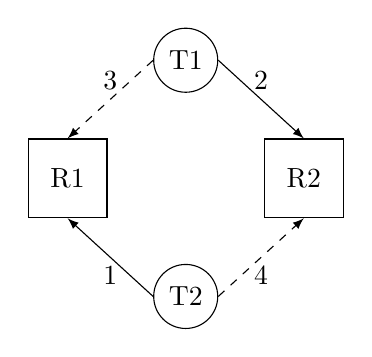
\begin{tikzpicture}
		\node[draw,rectangle,minimum height=1cm,minimum width=1cm] at (2,2.5) (r1) { R1 };
		\node[draw,rectangle,minimum height=1cm,minimum width=1cm] at (5,2.5) (r2) { R2 };
		\node[draw,circle,radius=0.5] at (3.5,1) (t2) { T2 };
		\node[draw,circle,radius=0.5] at (3.5,4) (t1) { T1 };

		\draw[-latex] (t2.west) -- node[below] {1} (r1.south);
		\draw[-latex]  (t1.east) -- node[above] {2} (r2.north);

		\draw[-latex,dashed] (t1.west) -- node[above] {3} (r1.north);
		\draw[-latex,dashed] (t2.east) -- node[below] {4} (r2.south) ;
	\end{tikzpicture}
\end{document}
